\documentclass[final,1p,times]{elsarticle}

\usepackage{amssymb}
\usepackage{amsmath,amsfonts}
\usepackage{algorithmic}
\usepackage{algorithm}
\usepackage{color,array}
\usepackage[caption=false,font=normalsize,labelfont=sf,textfont=sf]{subfig}
\usepackage{textcomp}
\usepackage{stfloats}
\usepackage{url}
\usepackage{verbatim}
\usepackage{graphics}
\usepackage{multirow}
\usepackage{bm}
\usepackage{threeparttable}
\usepackage{booktabs}
\usepackage{subfloat}
\usepackage{graphicx}

\renewcommand{\algorithmicrequire}{\textbf{Input:}}  
\renewcommand{\algorithmicensure}{\textbf{Output:}}
\newtheorem{myDef}{Definition}

%\journal{Expert Systems With Applications}

\bibliographystyle{model5-names}\biboptions{authoryear}

\begin{document}
	
	\begin{frontmatter}
		
		\title{Time-controlled incentive federated crowdsourcing}
		
		
		\author[mymainaddress]{Xiaoqian Jiang}
		\ead{220224926@seu.edu.cn}
		
		\author[mymainaddress]{Jing Zhang
			\corref{mycorrespondingauthor}}
		\ead{jingz@seu.edu.cn}
		
		\author[address2]{Cangqi Zhou}
		\ead{cqzhou@njust.edu.cn}
		
		\author[address3]{Ming Wu}
		\ead{mwu@hhu.edu.cn}
		
		\author[address4]{Victor S. Sheng}
		\ead{victor.sheng@ttu.edu}
		
		%\author[thirdaddress]{}
		%\ead{}
		
		\cortext[mycorrespondingauthor]{Corresponding author}
		\address[mymainaddress]{School of Cyber Science and Engineering, Southeast University, No. 2 SEU Road, Nanjing 211189, China}
		%\address[thirdaddress]{}
		\address[address2]{School of Computer Science and Engineering, Nanjing University of Science and Technology, No. 200 Xiaolingwei Street, Nanjing 210094, China}
		\address[address3]{School of Artificial Intelligence and Automation, Hohai University, No. 8 Fochengxi  Road, Nanjing 211100, China}
		\address[address4]{Department of Computer Science, Texas Tech University, Lubbock, TX 79409, USA}
		
		\begin{abstract}
			Crowdsourcing is an effective way to solve difficult tasks that cannot be solely solved by computers through a combination of human and machine intelligence. However, collecting data from massive crowdsourced workers for learning model training may expose them to the risk of privacy breaches because of the sharing of personal data, which will lower workers’ willingness to participate in crowdsourcing tasks. To address these issues, this paper introduces a federated learning paradigm and designs an incentive mechanism, namely TiFedCrowd, to mitigate the risk of privacy breaches for crowd workers and to obtain high-quality crowdsourcing data and learning models at the minimum cost. TiFedCrowd allows clients to keep privacy-related data locally. They just need to upload the trained models (parameters) to the server. The server then aggregates these uploaded models to train the global model. TiFedCrowd models the federated crowdsourcing process as a two-stage Stackelberg game to motivate more workers to complete crowdsourcing tasks with high quality and efficiency concurrently. At the same time, TiFedCrowd also defines a time control mechanism to manage the quality of the submitted models, the range of data freshness, and the waiting time for the data requester. TiFedCrowd requires the client to complete the federated crowdsourcing task within a specified time interval while maximizing the utility of both the clients and the server. We find the unique global optimal solution through the unique existence of Nash equilibrium. We also extended TiFedCrowd to the multiple heterogeneous federated crowdsourcing scenario. Extensive simulation shows that TiFedCrowd not only ensures the fairness of the incentive but also has significant effects on accelerating convergence speed, selecting data/model quality, and saving the budget of the data/model requester. Moreover, we also confirm the effectiveness of TiFedCrowd on real prediction tasks.
		\end{abstract}
		\begin{keyword}
			crowdsourcing learning, federated learning, privacy protection, incentive mechanism, Stackelberg game 
		\end{keyword}
	\end{frontmatter}

\section{Introduction}
Crowdsourcing provides a feasible way to introduce human intelligence to solve notoriously difficult tasks that cannot be solved by computers alone \citep{Vaughan2017MakingBU}. One of the most widespread applications of crowdsourcing is to collect data from massive Internet workers. The collected data including annotations, locations, content, and so on could be further utilized in downstream AI tasks such as building CV \citep{Kovashka2016CrowdsourcingIC}, NLP \citep{Wang2013PerspectivesOC}, recommendation \citep{Lin2023CompetitiveGI} models. Commercial crowdsourcing platforms such as MTurk, Appen, etc., have provided effective interaction modes between task publishers and workers to facilitate the execution of crowdsourced tasks. It is worth noting that while crowdsourcing provides convenience, it may also expose workers' privacy, which will reduce workers' willingness to participate in tasks. Prior research has shown that sensitive private information such as behavior traits, vocal prints, face images, and locations could be revealed along with the submitted data \citep{xia2020privacy,Tong2020FederatedLI}. Thus, privacy issues are attracting more and more attention in crowdsourcing task design. Some traditional approaches can achieve privacy protection by adding perturbation (e.g., implemented as differential privacy \citep{luo2016incentive,wang2022pps}) or noises \citep{to2018ppo,huang2020traffic}. Notwithstanding, these methods undermine the quality of crowdsourcing since the data uploaded by the workers are blurred.

Crowdsourcing platforms are the hubs for collecting data uploaded by workers. Thus, they are key parts of privacy security, where privacy leaks will affect massive crowdsourcing workers. In current crowdsourcing applications, there is a large class of tasks that collect data (usually annotations) from workers and use them in subsequent machine learning processes \citep{Sheng2019MachineLW}. With the increasing computation power of end devices and the fast growth of broadband networks, the model building can be directly performed on the end devices instead of being processed on the platform. That is, we can introduce federated learning (FL) \citep{mcmahan2017communication} to perform learning tasks. FL allows multiple distributed clients to collaborate on training shared models by iteratively aggregating model updates without exposing the raw data, which realizes privacy-preserving model training with little performance loss \citep{Yang2019FederatedML,Gao2022ASO}. Currently, FL has been fused with crowdsourcing and performs well in some situations \citep{Pandey2019ACF,Tong2020FederatedLI,zhang2021enabling}.

Although FL can effectively mitigate privacy breaches in crowdsourcing it also requires clients (i.e., workers in crowdsourcing) to contribute their data, computing, and communications resources, involving considerable costs. On the other hand, processing data locally on the client side indeed protects privacy. However, malicious attackers and the curious server still exist, who always struggle to probe the privacy lying the training samples from intermediate model parameters and gradients \citep{lyu2020threats,Song2020AnalyzingUP}. Such anxiety toward privacy security exacerbates participant inertia in FL \citep{mothukuri2021survey}. In addition, clients in FL have absolute control over their own devices, bandwidth, and data. That is, only the owners of clients can decide when, where, and how to participate in FL \citep{Liu2021FromDM}. Therefore, the incentive mechanism is very important for clients to participate in FL efficiently \citep{zhan2021incentive}. Unless clients can obtain enough compensation, they are unwilling to take those risks and contribute their resources. Sufficient incentives will encourage clients to respond optimally and eventually improve the performance of learned models.

Current incentive mechanisms in FL are usually designed around the driving factors of clients’ contribution, reputation, and resource allocation \citep{zhan2020learning,zhan2021survey}. Those incentive mechanisms designed for FL, targeting addressing the problems of how to accurately measure the contribution of each client and how to effectively attract and retain more clients, do not work well in crowdsourcing scenarios. The reasons are as follows: \lowercase{\romannumeral1}) In federated crowdsourcing, clients (workers) usually have the right to choose the human-intelligence tasks that are suitable for them. Thus, the incentive mechanism also needs to mobilize workers' interest and enthusiasm for crowdsourcing tasks. For example, it encourages clients to contribute more fresh data/models to keep the global model updated. \lowercase{\romannumeral2}) Due to the heterogeneity of clients' objective environments (e.g., computation ability of devices, communication bandwidth, and data resources) and subjective environments (e.g., expertise, dedication, and intention of workers), time control should be considered in federated crowdsourcing. On the one hand, the process of federated crowdsourcing is not necessarily as fast as possible. Platforms need time to assess the quality of submitted outcomes to prevent malicious workers from submitting low-quality data/model for quick rewards. On the other hand, the server (task publisher) must efficiently respond to delays in receiving data due to device and network failures as well as worker disruptions on client ends rather than waiting passively. \lowercase{\romannumeral3}) In federal crowdsourcing, platforms need to recruit and retain high-quality workers. Workers (clients) expect to be paid fairly and as high as possible. Task publishers (servers) expect to obtain as many high-quality outcomes as possible within their budget. Thus, the incentive mechanism of federated crowdsourcing must make a trade-off among these factors.

To address the above challenges, this paper puts forward \underline{Ti}me-controlled incentive \underline{Fed}erated \underline{Crowd}sourcing (TiFedCrowd), which inspires clients to complete data collection and local model training within the given time limit to optimize the global learning model. TiFedCrowd models the federated crowdsourcing process as a two-stage Stackelberg game \citep{li2017review} with a time limit. In the second stage (rewarding clients), TiFedCrowd allots rewards to clients based on their local model accuracies. Here, only the clients that upload models within the given time will be accepted and rewarded. Clients will adjust their model accuracies in the next round according to the costs of completing federated crowdsourcing tasks (mainly including the computing and communication costs) and the rewards obtained from the server. Through this adjustment, clients will be more proactive in taking on crowdsourcing tasks. In the first stage (maximizing the net utility of the server), TiFedCrowd sets a time interval on the server side to ensure the quality and efficiency of the server-side trained global model while maximizing the server-side net utility. The net utility is defined as the profit obtained by training the global model minus the total cost of incentivizing clients. In addition, only the models uploaded by the clients within the given time interval will be accepted and rewarded. Finally, we derive the Nash equilibrium in the Stackelberg game, which describes the steady state of the federated crowdsourcing process. The main contributions of the paper are as follows: 

\begin{itemize}
	\item We propose a novel time-controlled incentive federated crowdsourcing (TiFedCrowd), which encourages more workers to complete crowdsourcing tasks with high quality and efficiency as well as protects the privacy of participants. A time interval is set to preliminarily screen the quality of submitted outcomes. The upper bound of the interval enables the publisher (server-side) to specify the fresh level of the submissions, which is applicable to both instant and non-instant crowdsourcing.
	\item The Nash equilibrium of the Stackelberg game is derived. We prove that the Nash equilibrium of the proposed method can reach a  global maximization of the server and the client utilities. Furthermore, we prove the time interval theoretically improves the utility of the server and the performance of the global model.
	\item TiFedCrowd allocates rewards according to contributions, which has strong interpretability. It is conducive to attracting and retaining high-quality crowdsourcing workers, thus maintaining the fairness and accountability of the federated crowdsourcing market. TiFedCrowd also can be easily extended to multiple heterogeneous federated crowdsourcing tasks. A set of experiments on both simulated and real-world tasks was performed to show the effectiveness of TiFedCrowd.
\end{itemize}

The remainder of the paper is organized as follows: Section~\ref{sec:rw} briefly reviews the related studies.  Section~\ref{sec:mtd} presents the details of the proposed method. Section~\ref{tmh} demonstrates the generalization of TiFedCrowd to the multiple heterogeneous federated crowdsourcing scenario. Section~\ref{sec:exp} shows the experimental results and discusses them. Section~\ref{sec:con} concludes the paper with future work.

\section{Related Work}\label{sec:rw}
In this section, we briefly review the technical progress in two directions, i.e., privacy protection in crowdsourcing and incentive mechanism in federated learning.

\subsection{Privacy Protection in Crowdsourcing}
Since crowdsourcing usually involves collecting data from workers, it is inevitable that some tasks may touch workers' sensitive information. Thus, crowd workers face the risk of privacy disclosure \citep{xu2019blockchain,zhang2020decentralized}. Although differential privacy \citep{dwork2006differential} has been widely favored in the research field of Internet privacy protection since it was proposed, it works by injecting different levels of noise into the model. Undoubtedly, differential privacy will more or less sacrifice the accuracy of models \citep{bagdasaryan2019differential}. In addition, there are also techniques to protect the privacy of crowd workers that introduce various cryptographic algorithms. For example, \cite{shu2018privacy} proposed a privacy-preserving task recommendation scheme for crowdsourcing, which exploits polynomial functions to express multiple keywords of task requirements and worker interests, and then designed a key derivation method based on matrix decomposition. \cite{joshi2020salt} used SALT cryptography in the proposed solution to ensure privacy. \cite{zhang2019privacy} proposed a privacy-preserving traffic monitoring scheme through both adopting a homomorphic Paillier cryptosystem and super-increasing sequence. However, These encryption algorithms are complex, expensive, and cannot resist inference attacks \citep{lin2020secbcs,wang2019towards}.

To overcome the above defects, researchers introduced federated learning, which provides a secure way to work together so that participants can share and leverage data without exposing their privacy. For example, mean teacher semi-supervised FL \citep{zhang2021toward} introduces FL to provide a privacy-preserving framework for deep learning to realize the benefits of crowdsourcing. \cite{li2020crowdsf} proposed a crowdsourcing framework named CrowdSFL, which combines blockchain with FL to help users implement crowdsourcing with less overhead and higher security. These approaches to privacy protection in crowdsourcing by introducing the FL framework are all based on the ideal condition that participants are fully willing to make any contribution. However, FL usually requires considerable costs on the client's end. In most cases, crowd workers do not have such passions to contribute without enough rewards.

\subsection{Incentive Mechanism in Federated Learning}
An incentive mechanism is necessary to ensure the quality and efficiency of FL. The participation of clients in FL consumes computing resources, occupies network bandwidth, and even shortens the battery life of client devices. Clients are not willing to make sacrifices to participate in FL without any return. Accordingly, there is a growing body of research on the incentive mechanism of FL. \cite{zhan2020learn} designed a deep reinforcement learning-based incentive mechanism to determine the optimal pricing strategy for the parameter server and the optimal training strategies for edge nodes. \cite{le2021incentive} formulated the incentive mechanism between the base station and mobile users as an auction game and further proposed the primal-dual greedy auction mechanism to decide winners in the auction and maximize social welfare. \cite{zhang2021incentive} proposed an incentive mechanism of FL based on reputation and reverse auction theory, which selects and rewards participants by combining the reputation and bids of the participants under a limited budget.  \cite{9317806} modeled each data owner's contribution and the three categories of computing, communication, and privacy costs based on a multi-dimensional contract approach. \cite{pandey2019incentivize} introduced the crowdsourcing framework into FL and developed a two-stage Starkelberg game to maintain communication efficiency when participating clients implement uncoordinated computation strategy during aggregation of model parameters. \cite{kang2022incentive} proposed the incentive-boosted Federated Crowdsourcing and modeled the incentive-based interaction between the crowdsourcing platform and participating workers as a Stackelberg game to encourage workers to constantly collect fresh data.

Unfortunately, none of these incentive mechanisms works well in federated crowdsourcing that needs to collect data samples manually (i.e., so-call data crowdsourcing). Moreover, they all ignore the relationship between the time that workers collect data and the quality of submitted data in federated crowdsourcing and fail to respond to some delays in receiving data. The proposed TiFedCrowd in this study sets a time interval whose lower bound preliminarily screens the quality of submitted data and whose upper bound enables the task publisher to specify the fresh level of the data. Furthermore, the contribution of a worker is measured according to the accuracy \footnote{In this study, we simply use accuracy to measure the performance of learning models.} with which the client completes a local training model within the given time, and the rewards are fairly allocated in an economical manner, so as to motivate more workers to complete crowdsourcing tasks with high quality and efficiency.

\section{The Proposed TiFedCrowd Incentive Method} \label{sec:mtd}
In this section, we first present the federated crowdsourcing problem settings. Then, we present the proposed incentive mechanism as a two-stage Stackelberg game and also derive its equilibrium. Next, we summarize the whole process as an algorithm. Finally, we prove that time control is necessary for federated crowdsourcing.

\begin{figure}
	\centering
	\centerline{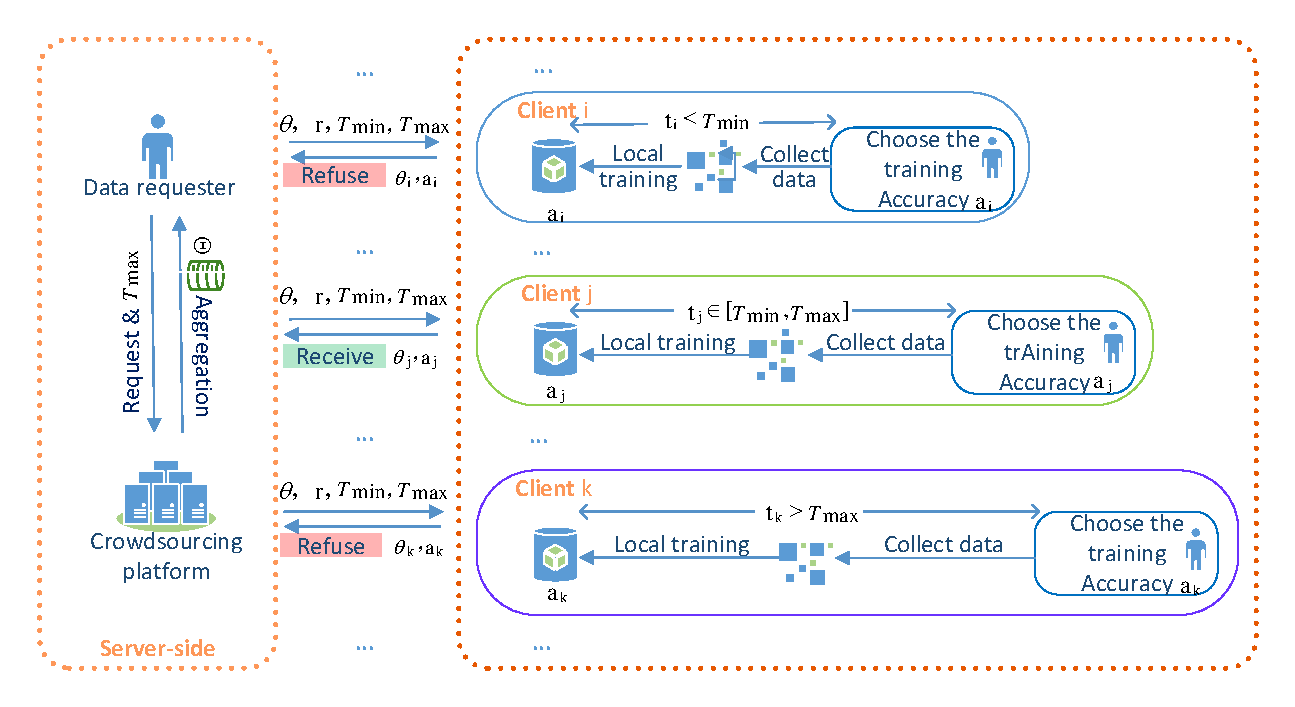
\includegraphics[width=5.5in]{TiFedCrowd framework.pdf}}
	\caption{Framework of the time-controlled incentive federated crowdsourcing (TiFedCrowd).}
	\label{fig:framework}
\end{figure}

\subsection{Problem Settings}
Let $\bm{\mathcal{N}} = \{1,2,\dots,n\}$ be a group of workers participating in federated crowdsourcing. For each worker $k\in\bm{\mathcal{N}}$, let $D_k=\{\bm{x_i}^k,y_i^k\}_{i=1}^m$ be the data sample set, where $m$ is the number of tasks, $\bm{x_i}^k\in\mathbb{R}^d$ is a vector with $d$ features representing the task for annotation, and $y_i^k\in\mathbb{R}$ is the label annotated for task $\bm{x_i}^k$ by worker $k$. To achieve privacy protection, TiFedCrowd requires that $D_k$ be kept locally and not shared with the server or other clients. In addition, each client trains its own local model $\theta_k$ through $D_k$ to collaboratively train the shared model $\Theta$.

Figure~\ref{fig:framework} shows the framework of the proposed TiFedCrowd model. The data requester first publishes task requirements and the allowed maximum completion time $T_{\max}$ through a crowdsourcing platform. Then, the platform (server) calculates the allowed minimum completion time $T_{\min}$ by evaluating task difficulty level and network quality and announces it to all clients along with the to-be-trained model $\theta$ and the reward rate $r$. For any client $k$, it determines his/her training accuracy level at the reward rate $r$. Next, the client collects data on demand to train the local model for attaining accuracy $a_k^\ast$ and sends the updated model to the server. Only those models uploaded within the time interval $[T_{\min},T_{\max}]$ will be accepted by the server, otherwise, they will be rejected. In this process, if the completion time of a model is greater than $T_{\max}$, it indicates that the local model updating may encounter some errors (i.e., network unavailable, training corrupt, data collection failed, etc.). The server will no longer receive the model. Another function of $T_{\max}$ is to control the fresh level of local models. The server will reject the local models whose completion times are greater than $T_{\max}$, deeming them outdated. If the completion time of a model is less than $T_{\min}$, it indicates that the client may not take the task seriously. The server also rejects it.  Finally, the server aggregates the received local models $\{\theta_k\}_{k=1}^n,T_k\in[T_{\min},T_{\max}]$ to obtain a global model and then distributes the rewards to clients whose models are successfully accepted according to the accuracy levels that they archived. 

The proposed TiFedCrowd aims to achieve a win-win situation using a novel incentive mechanism. Ideally, the server-side tries to encourage clients to contribute high-quality local models using as less as budget. whereas, the clients try to obtain more rewards by providing qualified outcomes within the specified time interval. Clearly, it is a gaming process. In the following sections, we will show that TiFedCrowd can reach an equilibrium status, where the utilities of both server and clients can be optimal. We will also show that introducing the time interval $[T_{\min}, T_{\max}]$ not only brings practical values (controlling the fresh levels of local models and filtering out low-quality local models) but also theoretically improves the utility of the server and the performance of the global model.

\subsection{Incentive Mechanism: The Two-Stage Stackelberg Game}
In the proposed time-controlled incentive federated crowdsourcing model, the data requester rewards clients who complete tasks within the specified time to achieve optimal local accuracy, thereby optimizing the global model. Simultaneously, upon receiving the rewards, rational clients will maximize their own profits respectively by improving the accuracy of the local models. We model such an interaction scenario as a two-stage Stackelberg game between a server (leader) and multiple clients (followers). In the Stackelberg game, both parties choose their own strategies based on the other's possible strategies to ensure that they maximize their interests under the other's strategy, so as to achieve the Nash equilibrium. The party that makes a decision first is called the leader. The remaining players (followers) make decisions based on the leader's decision. Then, the leader and followers adjust the initial decisions to make final better decisions by predicting the other party's response to their own decisions. The process is repeated until reaching the Nash equilibrium. 

Under our problem settings, the server first publishes local model requirements. Then, in Stage \uppercase\expandafter{\romannumeral2}, each client individually determines his/her own training accuracy according to the announced reward to maximize profit. After clients submit their work outcomes. In stage \uppercase\expandafter{\romannumeral1}, the server decides on the reward rate for clients to maximize the net utility and train the high-quality global model.

\textbf{Stage \uppercase\expandafter{\romannumeral2} (Clients):} In the client stage, the server will initially announce the uniform reward rate $r>0$ and time interval $[T_{\min},T_{\max}]$ for the participating clients. Rationally, for a client $k$, the reward $v_k$ is related to the accuracy level $a_k$ of the local model $\theta_k$. Intuitively, the higher the local accuracy level, the greater the revenue is:
\begin{equation}\label{eq:reward}
	v_k = r\cdot a_k\cdot \mathbb{I}(\tau),
\end{equation}
where $\mathbb{I}(\tau)$ is an indicator function that returns $1$ if the condition $\tau$ is true and $0$ otherwise. Only if the completion time $T_k$ meets condition $\tau: T_k\in[T_{\min},T_{\max}]$ will the model $\theta_k$ be accepted by the server and the reward $v_k$ be allocated. We refer to clients whose models are successfully accepted by the server as valid participants. Then, a rational worker will try to collect data to train a local model with high accuracy within the time limit for maximization of the revenue.  

Obviously, it inevitably brings costs $c_k$ for client $k$ to train a local model with a pre-defined accuracy on local data that can improve the global model. The costs include the computation cost $c_k^{comp}$ and the communication cost $c_k^{comm}$. That is, 
\begin{equation}\label{eq:cost}
	c_k	= c_k^{comp} + c_k^{comm}.
\end{equation}
Here, $c_k$ can be treated as the total cost of client $k$'s participation. The computation cost $c_k^{comp}$ is relevant to the number of iterations for training the local model $\theta_k$ to the target accuracy $a_k$. According to the relationship between iterations and accuracy in the local model training described in \citep{pandey2020crowdsourcing}, the computation cost of client $k$ is defined as follows:
\begin{equation}
	c_k^{comp} = \gamma_k\cdot \log(\frac{1}{1-a_k}),
\end{equation}
where $\gamma_k>0$ is a parameter choice of client $k$ that depends on the data size and condition number of the local subproblem \citep{konevcny2017semi}. Therefore, the more iterations of the local model training, the more computing resources the client spends.

The communication cost is related to the size of the model parameters and is incurred when the client interacts with the server for the model update. Since the to-be-trained model is published uniformly by the server, the total communication cost is the same for all clients as follows:
\begin{equation}
	c_k^{comm} = \lambda\cdot\xi,
\end{equation}
where $\lambda$ is a constant coefficient and $\xi$ represents the size of the model parameter.

Combining reward in Eq. (\ref{eq:reward}) and cost in Eq. (\ref{eq:cost}) of the client, for a valid participant, we define the utility of a client as follows:
\begin{equation}\label{eq:client-u}
	u_k = r\cdot a_k - c_k, \quad only\,\: if\quad\mathbb{I}(\tau) = 1.
\end{equation}

\textbf{Stage \uppercase\expandafter{\romannumeral1} (Server):} In the server stage of the game, the server can evaluate the optimal reward rate $r^\ast$ to maximize its net utility according to the response of valid participants. Let $\zeta$ be the number of valid participants, i.e.,
\begin{equation}
	\zeta = \sum_{k=1}^n\mathbb{I}(\tau).
\end{equation}
The utility of the server can be defined in relation to the maximum completion time of valid participants and the performance of the final global model achieved based on average local accuracy level. That is, 
\begin{equation}\label{Eq:server-u}
	U = \frac{1}{\zeta}\cdot \sum_{k=1}^n\left(\alpha\cdot a_k\cdot \mathbb{I}(\tau)\right) + \beta\cdot(T_{\max}-\max_{\mathbb{I}(\tau)=1,1\le k\le n}T_k) - \sum_{k=1}^n\left(r\cdot a_k\cdot \mathbb{I}(\tau)\right),
\end{equation}
where $\alpha > 0$ and $\beta \ge 0$ are system parameters, and $\sum_{k=1}^n(r\cdot a_k\cdot \mathbb{I}(\tau))$ is the cost totally spent for incentivizing clients that have validly participated in federated crowdsourcing. By default, we have $\beta = 0$, and $\beta > 0$ only makes sense in instant crowdsourcing (fresh data/model needs to be collected/trained constantly).

\subsection{Nash Equilibrium}
In this subsection, we will present the optimal solution to maximize the utility of both clients and the server by deducing the Nash equilibrium.

\begin{myDef}
	Nash Equilibrium. For any values of $r$ and $\bm{a}$, $(r^\ast,\bm{a}^\ast)$ is a Nash equilibrium if they satisfy the following conditions:
	\begin{equation}
		U(r^\ast,\bm{a}^\ast) \ge U(r,\bm{a}^\ast),
	\end{equation}	
	\begin{equation}
		u_k(r^\ast,a_k^\ast) \ge u_k(r^\ast,a_k),\, \forall k \in \bm{\mathcal{N}}.
	\end{equation}	
\end{myDef}

To find the equilibrium of the client stage in the game, we take the first derivative of $u_k(r,a_k)$ with respect to $a_k$ as follows:
\begin{equation}
	\frac{\partial u_k(r,a_k)}{\partial a_k} = r-\frac{\gamma_k}{1-a_k}.
\end{equation}	

Let $\frac{\partial u_k(r,a_k)}{\partial a_k} = 0$, we have
\begin{equation}\label{eq:a_k_ast}
	a_k^\ast = 1 - \frac{\gamma_k}{r}.
\end{equation}	

Then, we take the second derivative of $u_k(r,a_k)$ with respect to $a_k$ as follows:
\begin{equation}
	\frac{\partial^2 u_k(r,a_k)}{\partial a_k^2} = - \frac{\gamma_k}{(1-a_k)^2} < 0.
\end{equation}	

Hence, we derive and prove that $a_k^\ast = 1 - \frac{\gamma_k}{r}$ is the global optimal response accuracy of the client and is unique.

Since we have $0<a_k^\ast<1$, we can derive the value range of the reward rate $r$ as follows:
\begin{equation}
	0 < a_k^\ast = 1 - \frac{\gamma_k}{r} < 1\quad
	\Leftrightarrow\quad r > \gamma_k.
\end{equation}	

Based on the above derivations for clients (followers), as the leader in the game, the server can deduce the unique Nash equilibrium among valid participants for any reward rate $r>\gamma_k$. Accordingly, the server can choose the optimal reward rate $r^\ast$ to maximize its net utility. Based upon the sets of the completion time $\bm{T}^\ast$ and the optimum response accuracy $\bm{a}^\ast$, utility of the server is defined as follows:
\begin{equation}\label{eq:opt_u}
	U(r,\bm{a}^\ast) = \frac{1}{\zeta}\cdot \sum_{k=1}^n(\alpha\cdot a_k^\ast\cdot \mathbb{I}(\tau)) + \beta\cdot(T_{\max}-\max_{\mathbb{I}(\tau)=1,1\le k\le n}T_k^\ast) - \sum_{k=1}^n(r\cdot a_k^\ast\cdot \mathbb{I}(\tau)).
\end{equation}

Taking the first derivative of $U(r,\bm{a}^\ast)$ with respect to $r$, we obtain
\begin{equation}
	\begin{aligned}
		\frac{\partial U(r,\bm{a}^\ast)}{\partial r} &= \frac{1}{\zeta}\cdot \sum_{k=1}^n\left(\alpha\cdot \frac{\partial a_k^\ast}{\partial r}\cdot \mathbb{I}(\tau)\right) - \sum_{k=1}^n\left(r\cdot \frac{\partial a_k^\ast}{\partial r}\ast\cdot \mathbb{I}(\tau)\right) - \sum_{k=1}^n(a_k^\ast\cdot \mathbb{I}(\tau))\\&= \frac{\alpha}{\zeta\cdot r^2}\cdot\sum_{k=1}^n(\gamma_k\cdot\mathbb{I}(\tau))-\zeta.
	\end{aligned}
\end{equation}

Let $\frac{\partial U(r,\bm{a}^\ast)}{\partial r} = 0$, we have
\begin{equation}\label{eq:opt_r}
	r^\ast =\frac{1}{\zeta}\cdot\sqrt{\alpha\cdot\sum_{k=1}^n(\gamma_k\cdot\mathbb{I}(\tau))}.
\end{equation}	

The second derivative of $u_k(r,a_k)$ with respect to $r$ is as follows
\begin{equation}
	\frac{\partial^2 U(r,\bm{a}^\ast)}{\partial r^2} = - \frac{2\cdot\alpha}{\zeta\cdot r^3}\cdot\sum_{k=1}^n(\gamma_k\cdot\mathbb{I}(\tau)) < 0.
\end{equation}	

Therefore, we have proved that $r^\ast = \frac{1}{\zeta}\cdot\sqrt{\alpha\cdot\sum_{k=1}^n(\gamma_k\cdot\mathbb{I}(\tau))}$ is the global optimal reward rate and it is unique. 

To sum up, we have found the unique Nash equilibrium of the proposed incentive mechanism under federated crowdsourcing.

\subsection{Why Time Control Important}
To ensure the quality and efficiency of crowdsourcing, TiFedCrowd limits the time for the clients to complete the federated crowdsourcing tasks by setting a time interval $[T_{\min},T_{\max}]$. The upper bound $T_{\max}$ is set by the data/model requester according to his/her needs. $T_{\max}$ can make the server timely respond to the delays in receiving data which resulted from device and network failures as well as disruptions on clients rather than waiting passively. In addition, the completion deadline $T_{\max}$ also indicates the requester's recognition of the freshness of the data/models. In other words, as long as the data/models are submitted before $T_{\max}$, they are considered fresh. In addition, the completion deadline $T_{\max}$ also indicates the data requester's recognition of the freshness of the data. In other words, as long as the data submitted before $T_{\max}$ is considered fresh. The lower bound $T_{\min}$ is calculated by the server based on the task difficulty and network quality, which prevents malicious clients from submitting low-quality data/model for quick rewards. The ultimate goal of TiFedCrowd is to obtain a high-quality global model, based on which we demonstrate that time control is necessary for federal crowdsourcing.

Based on Eq.~(\ref{Eq:server-u}), we remove the time control in the definition of the server utility as follows: 
\begin{equation}
	\bar{U} = \frac{1}{n}\cdot \sum_{k=1}^n(\alpha\cdot a_k) + \beta\cdot(T_{\max}-\max_{1\le k\le n}T_k) - \sum_{k=1}^n(r\cdot a_k),
\end{equation}
where $\sum_{k=1}^n(r\cdot a_k)$ is the cost totally spent for incentivizing clients to participate in federated crowdsourcing. Apparently, the total cost $\sum_{k=1}^n(r\cdot a_k)$ for the server without time control is more than $\sum_{k=1}^n(r\cdot a_k\cdot \mathbb{I}(\tau))$ for one with time control.

To compare the magnitude of $\bar{U}$ and $U$, we take the difference between $\bar{U}$ and $U$:
\begin{equation}
	\bar{U} -U = \frac{1}{n}\cdot \sum_{k=1}^n(\alpha\cdot a_k)-\frac{1}{\zeta}\cdot \sum_{k=1}^n(\alpha\cdot a_k\cdot \mathbb{I}(\tau))- \beta\cdot(\max_{1\le k\le n}T_k-\max_{\mathbb{I}(\tau)=1,1\le k\le n}T_k) - \sum_{k=1}^n(r\cdot a_k\cdot (1-\mathbb{I}(\tau))).
\end{equation}

The completion time $T$ must satisfy the following derivation
\begin{equation}
	\max_{1\le k\le n}T_k\ge\max_{\mathbb{I}(\tau)=1,1\le k\le n}T_k\quad\Leftrightarrow\quad\beta\cdot(\max_{1\le k\le n}T_k-\max_{\mathbb{I}(\tau)=1,1\le k\le n}T_k)\ge0.
\end{equation}

For those data/models submitted after the deadline $T_{\max}$, whose freshness does not meet the requirements of the requester, we consider the accuracy level of their contributions to be $0$. Since TiFedCrowd uses the time control mechanism to filter out low-quality data/models, we have the following results:
\begin{equation}
	\begin{aligned}
		\frac{1}{n}\cdot \sum_{k=1}^n a_k < \frac{1}{\zeta}\cdot \sum_{k=1}^n\left( a_k\cdot \mathbb{I}(\tau)\right)\quad
		&\Leftrightarrow\quad \frac{1}{n}\cdot \sum_{k=1}^n(\alpha\cdot a_k)-\frac{1}{\zeta}\cdot \sum_{k=1}^n\left(\alpha\cdot a_k\cdot \mathbb{I}(\tau)\right)<0\\&\Leftrightarrow\quad  \bar{U} -U<0\quad\Leftrightarrow\quad  \bar{U} < U.
	\end{aligned}
\end{equation}	

In summary, we show that the server without time control has less utility and more incentivizing cost than the one with it. consequently, time control is critical to federated crowdsourcing.

\subsection{Algorithm}
The pseudo-code of TiFedCrowd is shown in Algorithm~\ref{Algo1}. Lines 2-13 are the procedures on the server side and lines 15-19 are for clients. Precisely, the process of the server side includes the following four steps: 1) estimate the minimum completion time (line 2); 2) calculate the optimum response accuracy at the given reward rate for each valid participant (lines 3-8); 3) computing the optimum reward rate, and announce it to clients, then wait until the deadline for them to complete the tasks (lines 10-12); 4) receive the updated models and return the aggregated global model (line 13).

The process of the client side includes the following three steps: 1) receive the task completion time interval and the declared reward rate from the server (line 15); 2) determine the optimum model accuracy and train a local model to achieve the accuracy within the specified time interval (lines 17-18); 3) send the trained local model to the server (line 19).

\begin{algorithm}[H]
	\caption{\underline {Ti}me-controlled incentive \underline{Fed}erated \underline{Crowd}sourcing (TiFedCrowd)}
	\label{Algo1}
	\begin{algorithmic}[1]
		\REQUIRE clients $\bm{\mathcal{N}} = \{1,2,\dots,n\}$; local data sample sets $\{D_k\}_{k=1}^n$; computation
		parameters $\{\gamma_k\}_{k=1}^n$; size of the published model $\xi$;  system parameters $\alpha$ and $\beta$; completion deadline $T_{\max}$.
		\ENSURE global learning model $\Theta$.\\
		\COMMENT{\textit{Procedure at the server}}
		\STATE Sever initializes the system parameters $\alpha$ and $\beta$ by the task type.
		\STATE Estimate the minimum completion time $T_{\min}$.
		\FOR{all clients $k = 1 \to n$ in parallel}
		\IF {completion time $T_k\in[T_{\min},T_{\max}]$}
		\STATE Compute the client $k$’s utility $u_k$ at the given reward rates $r$ via Eq. (\ref{eq:client-u}).
		\STATE Calculate the optimal response accuracy $a_k^\ast$ via Eq. (\ref{eq:a_k_ast}).
		\ENDIF
		\ENDFOR
		\STATE Compute the server’s utility via Eq. (\ref{eq:opt_u}).
		\STATE Choose the optimum reward rate $r^\ast$ via Eq. (\ref{eq:opt_r}), then announce it to all clients.
		\STATE Wait until time $T_{\max}$ for clients to complete the data collection and model training.
		\STATE Receive the updated models $\{\theta_k\}_{k=1}^n$ and send the rewards to valid participants based on their accuracy levels. Aggregate the global model $\Theta$.
		\RETURN the global model $\Theta$.\\
		\COMMENT{\textit{Procedure at client $k$}}
		\STATE Client initializes the computation
		parameter $\gamma_k$ according to the data size and condition number of the local subproblem.
		\STATE Receive the time interval $[T_{\min},T_{\max}]$ and the reward rate $r$.
		\STATE Compute the client utility $u_k$ via Eq. (\ref{eq:client-u}).
		\STATE Determine the training accuracy $a_k^\ast$ to solve the local subproblem via Eq. (\ref{eq:a_k_ast}).
		\STATE Collect the required data and train local model for attaining the accuracy level $a_k^\ast$ within the time interval $[T_{\min},T_{\max}]$.
		\RETURN the trained local model $\theta_k$ to the server.
	\end{algorithmic}
\end{algorithm}

The time complexity analysis of this algorithm needs to be discussed from the client side and the server side respectively. On the client side, the main time consumption of the algorithm is data collection and model training. The data collection time complexity is $O(m)$, where $m$ is the number of tasks collected by the client. The model training time complexity is $O(\log(a_k^{-1}))$, related to training the local model for attaining the accuracy $a_k$. Hence, the total time complexity of TiFedCrowd on the client side is $S[O(m)+O(\log(a_k^{-1}))]$. The space complexity is $O(\xi)$, where $\xi$ is the size of model parameters. On the server side, the main time consumption is to interact with the $n$ clients and the main space consumption is to aggregate the $n$ client models. Therefore, the time complexity of TiFedCrowd on the server side is $O(n)$ and the space complexity is $O(n\cdot\xi)$.

\section{TiFedCrowd for Multiple Heterogeneous Federated Crowdsourcing Tasks} \label{tmh}
In this section, we will show that TiFedCrowd can be easily extended to Multiple Heterogeneous Federated Crowdsourcing (MHFC) tasks. We first present the problem settings of MHFC tasks. Then, we model TiFedCrowd for MHFC as a two-stage Stackelberg game. Finally, we derive the Nash equilibrium for the model.

\subsection{Problem Settings of MHFC Tasks}
In Section~\ref{sec:mtd}, we have an underlying assumption that the requester has divided the task into subtasks with equal (or approximately equal) completion costs. This setting is a better choice in most federated crowdsourcing applications because it has a simple protocol for quality control and reward distribution. However, there are still some crowdsourcing tasks in reality, and it is difficult for them to be evenly divided. For example, some classification tasks may have a very imbalanced distribution of underlying classes. Then, for workers participating in federated crowdsourcing tasks, it is difficult for them to collect samples with a similar distribution. That is, some workers may spend a lot of effort collecting samples in rare categories, while others collect those in majority categories with ease. Therefore, the costs of workers collecting data, training models, and submitting models vary significantly. We call this scenario as the multiple heterogeneous federated crowdsourcing.

Let $\{\Omega^{(i)}\}_{i=1}^s$ be a set of heterogeneous federated crowdsourcing tasks, where $s$ is the number of types of tasks. Tasks of the same type have approximately the same cost. The requester first publishes task requirements and an allowed maximum completion time $T_{\max}$ for all types of tasks. Here, we set the only $T_{\max}$ because the requester usually publishes a unique deadline for all submissions. Let $\{\bm{\mathcal{N}}^{(i)}\}_{i=1}^s$ be $s$ groups of workers participating in the tasks. Workers in group $i$ (for the tasks with type $i$) are $\bm{\mathcal{N}}^{(i)} = \{1^{(i)},2^{(i)},\dots,n^{(i)}\}$, whose elements are serial numbers for the workers. That is, $n^{(i)}$ happens to be the number of workers involved in tasks $\Omega^{(i)}$. The server calculates the minimum completion times $\{T_{\min}^{(i)}\}_{i=1}^s$ for all types of tasks by jointly evaluating the difficulties of different types of tasks and the network qualities. Then, the server announces them to all clients along with the to-be-trained models $\{\theta^{(i)}\}_{i=1}^s$ and the reward rates $\{r^{(i)}\}_{i=1}^s$. The reward rate $r^{(i)}$ varies by the type of tasks $\Omega^{(i)}$, which can prevent clients from selecting only simple tasks. Finally, let $\{\xi^{(i)}\}_{i=1}^s$ be the sizes of the parameters of these types of learning models.

\subsection{The Two-Stage Stackelberg Game for MHFC}
\textbf{Stage \uppercase\expandafter{\romannumeral2} (Clients):} A client $k^{(i)}\in\bm{\mathcal{N}}^{(i)}\subseteq\{\bm{\mathcal{N}}^{(i)}\}_{i=1}^s$ tries to collect data on demand to train the local model for attaining accuracy ${a_k^{(i)}}^\ast$ and sends the updated model $\theta_k^{(i)}$ to the server within the time interval $[T_{\min}^{(i)},T_{\max}]$ to collaboratively train the shared model $\Theta$. Therefore, for a valid participant whose completion time $T_k^{(i)}$ meets condition $\tau^{(i)}:T_k^{(i)}\in[T_{\min}^{(i)},T_{\max}]$, we define the utility of client $k^{(i)}$ in task type $i$ as follows:
\begin{equation}
	u_k^{(i)} = r^{(i)}\cdot a_k^{(i)} - c_k^{(i)}, \quad only\,\: if\quad\mathbb{I}(\tau^{(i)}) = 1.
\end{equation}
Here, $c_k^{(i)}$ is the total cost of the participation of client $k^{(i)}$:
\begin{equation}
	c_k^{(i)} = \gamma_k^{(i)}\cdot \log(\frac{1}{1-a_k^{(i)}})+\lambda\cdot\xi^{(i)},
\end{equation}
where $\gamma_k^{(i)}\cdot \log(\frac{1}{1-a_k^{(i)}})$ is the computation cost and $\lambda\cdot\xi^{(i)}$ is the communication cost.

\textbf{Stage \uppercase\expandafter{\romannumeral1} (Server):} The utility of the server in TiFedCrowd for MHFC tasks can be defined as follows:
\begin{equation}
	\mathcal{U} = \frac{1}{\zeta}\cdot \sum_{i=1}^{s}\sum_{k=1}^{n^{(i)}}\left(\alpha^{(i)}\cdot a_k^{(i)}\cdot \mathbb{I}(\tau^{(i)})\right) + \beta\cdot(T_{\max}-\max_{\mathbb{I}(\tau^{(i)})=1,1\le k\le n^{(i)},1\le i\le s}T_k^{(i)}) - \sum_{i=1}^{s}\sum_{k=1}^{n^{(i)}}\left(r^{(i)}\cdot a_k^{(i)}\cdot \mathbb{I}(\tau^{(i)})\right),
\end{equation}
where the system parameters $\{\alpha^{(i)}\}_{i=1}^s$ ($\alpha^{(i)}>0$) also can  represent the weights of multiple heterogeneous tasks and $\sum_{i=1}^{s}\sum_{k=1}^{n^{(i)}}\left(r^{(i)}\cdot a_k^{(i)}\cdot \mathbb{I}(\tau^{(i)})\right)$ is the total cost for incentivizing clients that have validly participated in federated crowdsourcing. In addition, the number of valid participants $\zeta$ is calculated as follows:
\begin{equation}
	\zeta = \sum_{i=1}^{s}\sum_{k=1}^{n^{(i)}}\mathbb{I}(\tau^{(i)}).
\end{equation}

\subsection{Nash Equilibrium for MHFC in TiFedCrowd}
\begin{myDef}
	Nash Equilibrium for MHFC Tasks. For any values of $\bm{r}$ and $\bm{A}$, $(\bm{r}^\ast,\bm{A}^\ast)$ is a Nash equilibrium for MHFC tasks if they satisfy the following conditions:
	\begin{equation}
		\mathcal{U}(\bm{r}^\ast,\bm{A}^\ast) \ge \mathcal{U}(\bm{r},\bm{A}^\ast),
	\end{equation}	
	\begin{equation}
		u_k^{(i)}({r^{(i)}}^\ast,{a_k^{(i)}}^\ast) \ge u_k^{(i)}({r^{(i)}}^\ast,a_k^{(i)}),\, \forall k^{(i)}\in\bm{\mathcal{N}}^{(i)}\subseteq\{\bm{\mathcal{N}}^{(i)}\}_{i=1}^s.
	\end{equation}	
\end{myDef}

To find the equilibrium for MHFC tasks of the client stage in the game, let the first derivative of $u_k^{(i)}(r^{(i)},a_k^{(i)})$ with respect to $a_k^{(i)}$ be $0$, we have:
\begin{equation}
	\frac{\partial u_k^{(i)}(r^{(i)},a_k^{(i)})}{\partial a_k^{(i)}} = r^{(i)}-\frac{\gamma_k^{(i)}}{1-a_k^{(i)}} = 0 \quad
	\Leftrightarrow\quad {a_k^{(i)}}^\ast = 1 - \frac{\gamma_k^{(i)}}{r^{(i)}}.
\end{equation}	
Since the second derivative of $u_k^{(i)}(r^{(i)},a_k^{(i)})$ with respect to $a_k^{(i)}$ is
\begin{equation}
	\frac{\partial^2 u_k^{(i)}(r^{(i)},a_k^{(i)})}{\partial {a_k^{(i)}}^2} = - \frac{\gamma_k^{(i)}}{(1-a_k^{(i)})^2} < 0,
\end{equation}	
${a_k^{(i)}}^\ast = 1 - \frac{\gamma_k^{(i)}}{r^{(i)}}$ is the unique global optimal response accuracy of the client.

According to $0<{a_k^{(i)}}^\ast<1$, the value range of the reward rate $r^{(i)}$ is derived as follows:
\begin{equation}
	0 < {a_k^{(i)}}^\ast = 1 - \frac{\gamma_k^{(i)}}{r^{(i)}} < 1\quad
	\Leftrightarrow\quad r^{(i)} > \gamma_k^{(i)}, \quad i=1,2,\dots,s.
\end{equation}	

Based on the sets of the completion time $\bm{T}^\ast$ and the optimum response accuracy $\bm{A}^\ast$, the utility of the server for MHFC tasks can be defined as follows:
\begin{equation}
	\mathcal{U}(\bm{r},\bm{A}^\ast) = \frac{1}{\zeta}\cdot \sum_{i=1}^{s}\sum_{k=1}^{n^{(i)}}\left(\alpha^{(i)}\cdot {a_k^{(i)}}^\ast\cdot \mathbb{I}(\tau^{(i)})\right) + \beta\cdot(T_{\max}-\max_{\mathbb{I}(\tau^{(i)})=1,1\le k\le n^{(i)},1\le i\le s}{T_k^{(i)}}^\ast) - \sum_{i=1}^{s}\sum_{k=1}^{n^{(i)}}\left(r^{(i)}\cdot {a_k^{(i)}}^\ast\cdot \mathbb{I}(\tau^{(i)})\right).
\end{equation}
Then, let the first derivative of $U(\bm{r},\bm{A}^\ast)$ with respect to $\bm{r}$ be $0$, we obtain
\begin{equation}
	\begin{aligned}
		\frac{\partial \mathcal{U}(\bm{r},\bm{A}^\ast)}{\partial r^{(i)}} &= \frac{1}{\zeta}\cdot \sum_{k=1}^{n^{(i)}}\left(\alpha^{(i)}\cdot \frac{\partial {a_k^{(i)}}^\ast}{\partial r^{(i)}}\cdot \mathbb{I}(\tau^{(i)})\right) - \sum_{k=1}^{n^{(i)}}\left( r^{(i)}\cdot \frac{\partial {a_k^{(i)}}^\ast}{\partial r^{(i)}}\ast\cdot \mathbb{I}(\tau^{(i)})\right) - \sum_{k=1}^{n^{(i)}}\left({a_k^{(i)}}^\ast\cdot \mathbb{I}(\tau^{(i)})\right)\\
		&= \frac{\alpha^{(i)}}{\zeta\cdot {r^{(i)}}^2}\cdot\sum_{k=1}^{n^{(i)}}\left(\gamma_k^{(i)}\cdot\mathbb{I}(\tau^{(i)})\right)-\zeta = 0\\
		&\Leftrightarrow\quad {r^{(i)}}^\ast =\frac{1}{\zeta}\cdot\sqrt{\alpha^{(i)}\cdot\sum_{k=1}^{n^{(i)}}\left(\gamma_k^{(i)}\cdot\mathbb{I}(\tau^{(i)})\right)}, \quad i=1,2,\dots,s.
	\end{aligned}
\end{equation}
Taking the second derivative of $U(\bm{r},\bm{A}^\ast)$ with respect to $\bm{r}$, we have
\begin{equation}
	\frac{\partial^2 \mathcal{U}(\bm{r},\bm{A}^\ast)}{\partial {r^{(i)}}^2} = - \frac{2\cdot\alpha^{(i)}}{\zeta\cdot {r^{(i)}}^3}\cdot\sum_{k=1}^{n^{(i)}}\left(\gamma_k^{(i)}\cdot\mathbb{I}(\tau^{(i)})\right) < 0.
\end{equation}	
Hence, ${r^{(i)}}^\ast =\frac{1}{\zeta}\cdot\sqrt{\alpha^{(i)}\cdot\sum_{k=1}^{n^{(i)}}\left(\gamma_k^{(i)}\cdot\mathbb{I}(\tau^{(i)})\right)}$ ($i=1,2,\dots,s$) are the unique global optimal reward rates for all types of tasks.

We have derived the Nash equilibrium for MHFC tasks in TiFedCrowd. This is not difficult for us to write an algorithm that is similar to Algorithm~\ref{Algo1}, which can solve the incentive problem of MHFC tasks.

\section{Experiments} \label{sec:exp}
This section presents the experiments and discussions on the results. First, we present our experimental setup. Then, we present the comparison results on the simulated incentive process between clients and the server as well as the results of ablation experiments. Finally, we show the experimental results on a real-world dataset.

\subsection{Experimental Setup}
To comprehensive evaluation the performance of the proposed method. We conduct a set of simulations to compare our proposed method with some existing methods.
\paragraph{\textbf{Simulation Process}}
We set the number of participating clients $n$ and the completion time interval $[T_{\min},T_{\max}]$ to $30$ and $[5,30]$ (unit: second) respectively. Besides, we initialized the utility of the server with the parameters $\alpha=300$ and $\beta=0$. Nevertheless, any reasonable settings for these values would not affect the comparisons on performance. 
\paragraph{\textbf{Methods Used in Comparison}}
Among the existing incentive mechanical design of federated crowdsourcing, we have not found a method having the same rules of the game as our TiFedCrowd. We each have different purposes so that the definitions of utility in our method vary. Such as, \cite{pandey2019incentivize} is aiming to minimize the communication cost between server and clients, \cite{kang2022incentive} is aiming to encourage workers to constantly collect fresh data. While we aim to obtain a more accurate global model at a lower cost. Therefore, none of them are suitable for comparison with TiFedCrowd. As with \cite{pandey2019incentivize} and \cite{kang2022incentive}, we also compare the incentive mechanism in our TiFedCrowd to the baselines. Our baselines are:
\begin{itemize}
	\item RWD\_MAX: Always select the largest reward rate ($r$) to obtain the best response from clients.  
	\item RWD\_MIN: Always pick the smallest reward rate ($r$) to minimize the total incentive cost on the server-side.
	\item RWD\_RAND: Randomly choose the reward rate ($r$) to motivate the clients.
\end{itemize}

\paragraph{\textbf{Evaluation Metrics}}
We set four evaluation metrics to evaluate the performance of TiFedCrowd from different perspectives. Our evaluation metrics are: reward rate ($r$), average utility of clients, utility of the server, and total incentive cost. 
\subsection{Comparison Results on Simulated Experiment} \label{PCWB}
Since the number of valid participants within a reasonable range would not affect the comparison results in this section, we assumed that all clients validly participate in federated crowdsourcing tasks (i.e., the completion time $T_k\in[T_{\min},T_{\max}],\,\forall k\in\bm{\mathcal{N}}$).
We compared at different client parameter $\gamma$ the performance between TiFedCrowd and the baselines to illustrate that our method is efficient. Therefore, we let $\gamma$ be uniformly distributed randomly in intervals $[\Delta, \Delta + 0.5]$ ($\Delta = 1.0, 1.5, 2.0, 2.5, 3.0, 3.5$) to analyze the impact of the client parameter $\gamma$.

\begin{figure}
	\centering
	\centerline{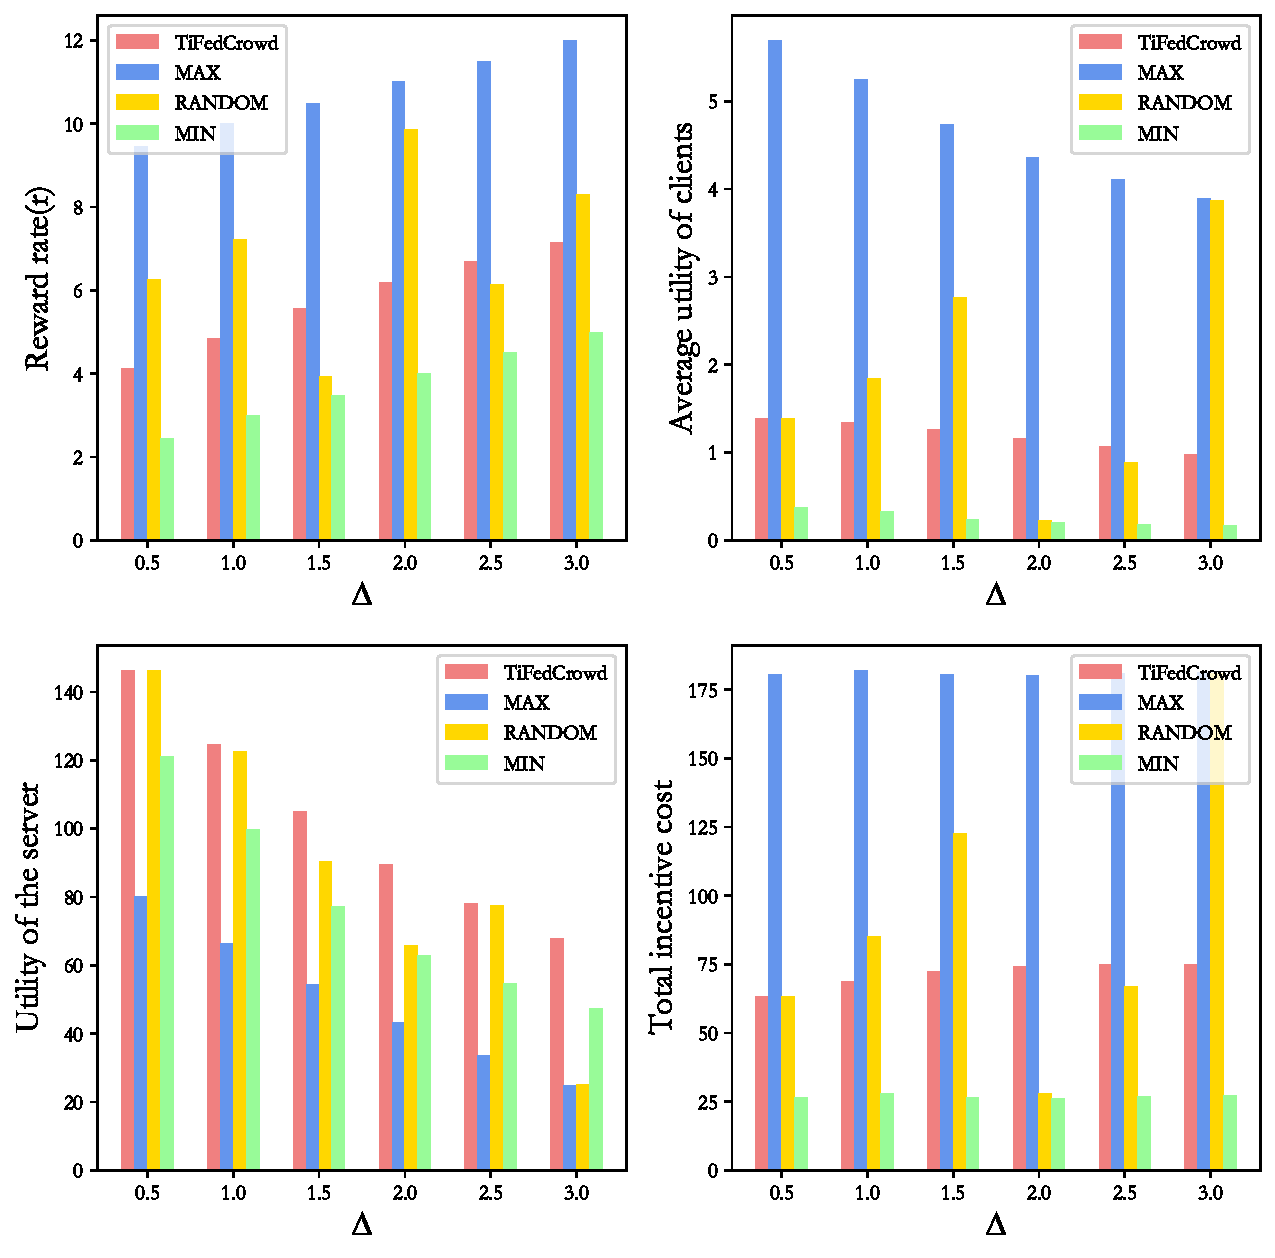
\includegraphics[width=5.5in]{fig2.pdf}}
	\caption{Reward rate ($r$), average utility of clients, utility of the server, and total incentive cost vs. client parameter $\gamma$ ($\gamma\in[\Delta,\Delta+0.5]$).}
	\label{fig:2}
\end{figure}

Figure~\ref{fig:2} respectively reports under different client parameters $\gamma$ the reward rate ($r$), the average utility of clients, the utility of the server, and the total incentive cost of TiFedCrowd and the baselines. It is not hard to observe the competition between  clients and the server that the higher the reward rate ($r$), the greater the average utility of clients while the less the utility of the server. Besides, we have other observations as follows: 

\lowercase{\romannumeral1}) With the increase of client parameter $\gamma$, the reward rate ($r$) of TiFedCrowd, RWD\_MAX, and RWD\_MIN also increases steadily, while the reward rate ($r$) of RWD\_RAND distributes randomly within the range of RWD\_MIN and RWD\_MAX. This is because the larger customer parameter $\gamma$ brings the higher cost for the clients to participate in federated crowdsourcing so greater incentives are needed to motivate the participation of the clients.

\lowercase{\romannumeral2}) Among these four methods, RWD\_MAX always has the most average utility of clients while RWD\_MIN always has the least. After all, MAX chooses the largest reward rate to motivate the client while RWD\_MIN selects the smallest one. Besides, the average utility of clients of TiFedCrowd, RWD\_MAX, and RWD\_MIN decreases as the client parameter $\gamma$ gets larger. Since the increase of the client parameter $\gamma$ means that the clients have to spend more cost to complete the federated crowdsourcing tasks, their profits inevitably reduce. Moreover, except for RANDOM, the utility of the server of TiFedCrowd, RWD\_MAX, and RWD\_MIN becomes less and less as the client parameter $\gamma$ increases. The reason is that the larger client parameter $\gamma$ leads to the higher cost of the client to complete the federated crowdsourcing tasks, so the client will appropriately reduce the local training accuracy to reduce the computational cost to maximize its utility.

\lowercase{\romannumeral3}) TiFedCrowd results in the highest utility of the server among the four methods whatever the value of the client parameter $\gamma$ because TiFedCrowd always incentivizes the client with the optimum reward rate to maximize the utility of the server. However, the utility of the server of RWD\_MAX is always the lowest. And it is easy to understand that RWD\_MAX always incentivize clients with the highest reward rate, which greatly increases the total cost of the server. In addition, the utility of the server of RWD\_MIN is higher than it of RWD\_MAX all the time. Although RWD\_MIN minimizes the total cost on the server-side by incentivizing clients with the minimal reward rate, it also causes the clients to upload low-quality models thus reducing the utility of the server. 

\lowercase{\romannumeral4}) The total incentive cost of RWD\_MAX, RWD\_MIN, and TiFedCrowd almost does not change with different client parameter $\gamma$. This means that how much clients spend in completing the federated crowdsourcing tasks does not affect the total incentive cost on the server-side when the number of valid participants is fixed.

\lowercase{\romannumeral5}) Although randomly selecting the reward rate to incentivize the clients in RWD\_RAND brings good utility to both the clients and the server, randomizing the reward results in a higher reward for submitting a low-quality model while a lower reward for submitting a high-quality model. This not only breaks the fairness of the crowdsourcing market but also makes it is no interpretability, which is not conducive to long-term cooperation between clients and crowdsourcing platforms.

All above observations illustrate that TiFedCrowd can maximize the utility of the server side with as little cost as possible on the premise of ensuring the fairness of the crowdsourcing market and the interpretability of the incentive mechanism.

\subsection{Impact of the Number of Clients}\label{ITNC}
Since the number of clients participating in the federated crowdsourcing tasks directly determines the degree of competition in the crowdsourcing market, it indirectly affects the quality of data/models collected on the server-side. In this subsection, We further studied the impact of the number of clients on the performance of TiFedCrowd. To analyze the number of clients alone, we assumed that all clients of the experiments in this subsection were valid participants (i.e., the completion time $T_k\in[T_{\min},T_{\max}],\,\forall k\in\bm{\mathcal{N}}$). As the number of clients exceeds $35$, the comparison results tend to be in a balanced state. Therefore, in Figure~\ref{fig:4}, we plotted the reward rate ($r$), the average utility of clients, the utility of the server, and the total incentive cost in TiFedCrowd compared to them in baselines as the number of clients increases from $15$ to $35$. We have the following observations:

\begin{figure}
	\centering
	\centerline{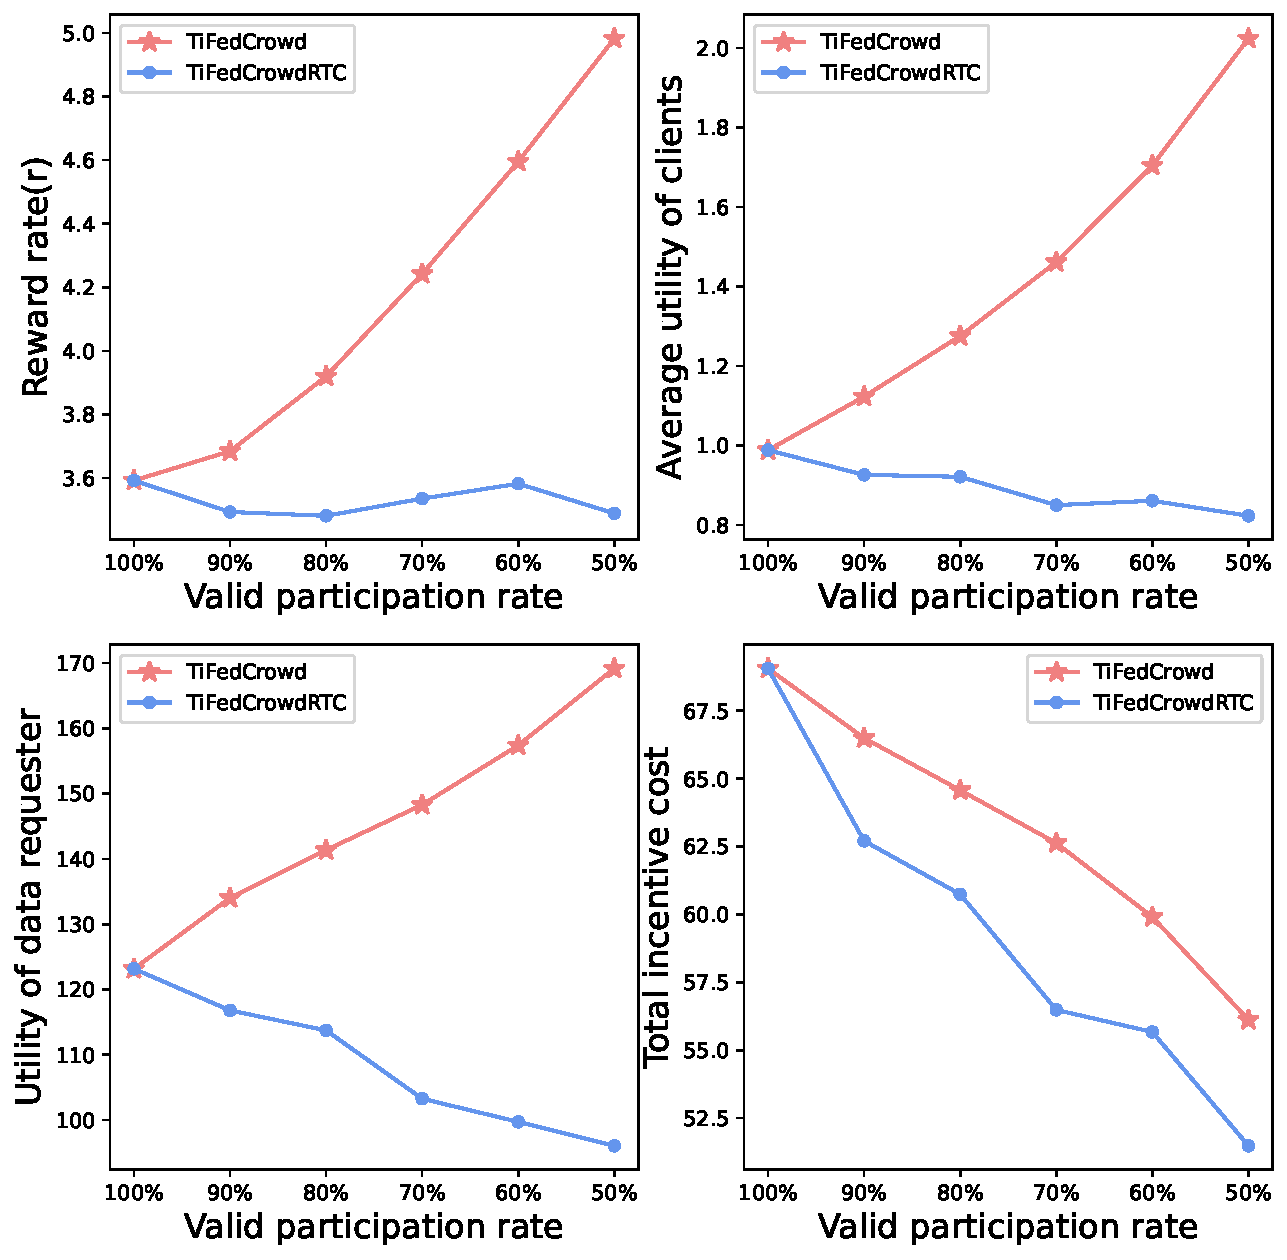
\includegraphics[width=5.5in]{fig4.pdf}}
	\caption{Reward rate ($r$), average utility of clients, utility of the server, and total incentive cost vs. number of clients.}
	\label{fig:4}
\end{figure}

 \lowercase{\romannumeral1}) The reward rate ($r$) and the average utility of clients have the similar changing trend as the number of clients varies. According to Eq.~(\ref{eq:reward}), we define in TiFedCrowd that the rewards a client receives is proportional to the accuracy it contributes. Based on Eq.~(\ref{eq:a_k_ast}), and because we controlled that the client parameters $\{\gamma_k\}_{k=1}^n$ were uniformly distributed in a small interval, the accuracy difference of these clients contribution was small under the uniformly declared reward rate ($r$) of the server. So did the cost they spend based on Eq.~(\ref{eq:cost}). Therefore, as the variation of the number of clients, the changing trend of the reward rate ($r$) and the average utility of clients is almost the same in Figure~\ref{fig:4}. Besides, RWD\_MAX always has the highest reward rate ($r$). RWD\_MIN always has the lowest reward rate ($r$). The reward rate ($r$) of RWD\_RAND and TiFedCrow is always between RWD\_MIN and RWD\_MAX. According to the way they select the reward rate ($r$), such magnitude relationship of the reward rate ($r$) in these four methods remains the same regardless of how the number of clients varies. So does the average utility of clients since it always has a similar change trend as the reward rate ($r$). In addition, in RWD\_MAX and RWD\_MIN, the reward rate ($r$) and the average utility of clients are always maintained near the constant value and do not fluctuate with the variation of the number of clients because the selection of the reward rate ($r$) of RWD\_MAX and RWD\_MIN depends only on the reasonable range of $r$ and not on the number of clients. The reward rate ($r$) and the average utility of clients in TiFedCrowd get smaller and smaller as the number of clients increases. This is because TiFedCrowd always selects the optimum reward rate ($r$) to motivate the clients to maximize the utility of the server. With the increasing number of participating clients, the server-side has to reduce the incentive effort to save the total incentive cost and ensure the maximum utility of the server. In addition, more clients participating in the competition also cause the average utility of the clients to decline. 
 
 \lowercase{\romannumeral2}) In all four methods, the utility of the server declines as the number of clients increases because of the increase in the total incentive cost spent by the server. Besides, the utility of the server in TiFedCrowd and RWD\_MIN decreases slowly while in RWD\_MAX sharply. TiFedCrowd continually adjusts the incentives to maximize the utility of the server. RWD\_MIN always incentivizes the clients with minimal effort while RWD\_MAX with maximal. RWD\_MAX obviously causes serious waste of budget. Besides, the utility of the server of TiFedCrowd is always the highest among the four methods. Although the utility of the server of RWD\_MIN is only slightly lower than TiFedCrowd, RWD\_MIN achieves a high level of utility of the server in a way that minimizes the total incentive cost on the server side. Therefore, The method of RWD\_MIN may not only reduce the accuracy of the global model but also increase the reluctance of the clients to participate, which is undesirable.
 
 \lowercase{\romannumeral3}) The total incentive cost aggrandizes for all four methods as the number of clients increases. Relate to what we observed in subsection~\ref{PCWB}, the cost of the clients to complete the federated crowdsourcing tasks does not affect the total incentive cost on the server-side when the number of the valid participants is fixed. Therefore, the number of valid participants is the direct influence on the total incentive cost on the server-side.

 \lowercase{\romannumeral4}) Comprehensive reward rate ($r$), the average utility of clients, the utility of the server, and the total incentive cost, the method of RWD\_RAND is much more flexible compared to other methods. However, as we analyzed in section subsection~\ref{PCWB}, the method of RWD\_RAND breaks the fairness of the crowdsourcing market as well as compromises the long-term cooperation between clients and crowdsourcing platforms.

\subsection{Comparison of Convergence Speed} \label{CTCT}
In subsection~\ref{ERCP}, we compared our TiFedCrowd to iFedCrowd \citep{kang2022incentive} which is the state-of-the-art incentive mechanism for federated crowdsourcing as well as the closest method to our TiFedCrowd. However, our TiFedCrowd is superior to iFedCrowd not only because we use the time control mechanism to screen out low-quality data. In this subsection, we performed experiments to show that our TiFedCrowd has a shorter computing time than iFedCrowd. 

We compared the time for the server to calculate the reward rate ($r$) each time in both methods TiFedCrowd and iFedCrowd. Table~\ref{tab:t2} records the run time of 1000 executions for each of the two methods varying the number of clients. The hardware configuration used for our calculations is Intel(R) core(TM) i5, 8G.

\begin{table}
	\caption{The time (the measuring unit: second) for the server to calculate the reward rate ($r$)}
	\centering
	\setlength{\tabcolsep}{8mm}{ 
		\begin{tabular}{ccc} 
			\toprule
			\textbf{ The number of clients } & \textbf{ TiFedCrowd }  & \textbf{ iFedCrowd }      \\ 
			\hline
			10     & 0.022 & 0.872  \\
			100    & 0.022 & 1.899  \\
			500    & 0.022 & 6.779 \\
			1000   & 0.028 & 12.969 \\
			5000   & 0.042 & 69.516 \\ 
			10000  & 0.061 & 138.364  \\
			\bottomrule
	\end{tabular}}
	\label{tab:t2}
\end{table}

As the number of clients increases, the computing time of TiFedCrowd changes very slowly. Even if the number of clients is scaled up to 1000 times, the computing time of TiFedCrowd is scaled up to less than 3 times. On the contrary, the computation time of iFedCrowd obviously increases with the number of clients. When the number of clients grew from 10 to 1,0000, iFedCrowd's compute time expands by more than 100 times. The larger the number of clients, the greater the advantage of TiFedCrowd over iFedCrowd in computing time. When the number of clients is 10, the computation time of TiFedCrowd is $2.5\%$ of iFedCrowd. However, when the number of clients grows to 10000, the computing time of TiFedCrowd is only $0.04\%$ of iFedCrowd, which saves a lot of time on the server-side. All these observation results from table~\ref{tab:t2} show that our TiFedCrowd has a huge advantage over iFedCrowd in terms of computation time for the reward rate ($r$). Coupled with the time control mechanism that stipulates the task completion deadline, TiFedCrowd makes the convergence time of the whole crowdsourcing project shorter.

\subsection{Ablation Experiment of Time Control}\label{RTTCM}
To manifest the effectiveness of the time control mechanism in TiFedCrowd, we compared the performance between TiFedCrowd and which removed time control (RTC). In the experiments of this section, we fixed the client parameter $\gamma\in[1.0,1.5]$. Since the upper bound $T_{\max}$ of the time interval $[T_{\min},T_{\max}]$ is set subjectively by the data/models requster, the evaluation criteria of its screening effect on the quality of the collected data depends on the setter's subjective satisfaction. Here we assumed that the completion time $T$ for all clients satisfy the constraint $T_{\max}$ (i.e, $T_k\le T_{\max},\,\forall k\in\bm{\mathcal{N}}$) while researching the screening effect of the lower bound $T_{\min}$ on the quality of the collected data. To investigate the effect of the valid participation rate (the percentage of valid participants (i.e., $T_k\in [T_{\min},T_{\max}],\, k\in\bm{\mathcal{N}}$) among all participating clients), we set the valid participation rate for six gradients: $100\%$, $90\%$, $80\%$, $70\%$, $60\%$, $50\%$. 

\begin{figure}
	\centering
	\centerline{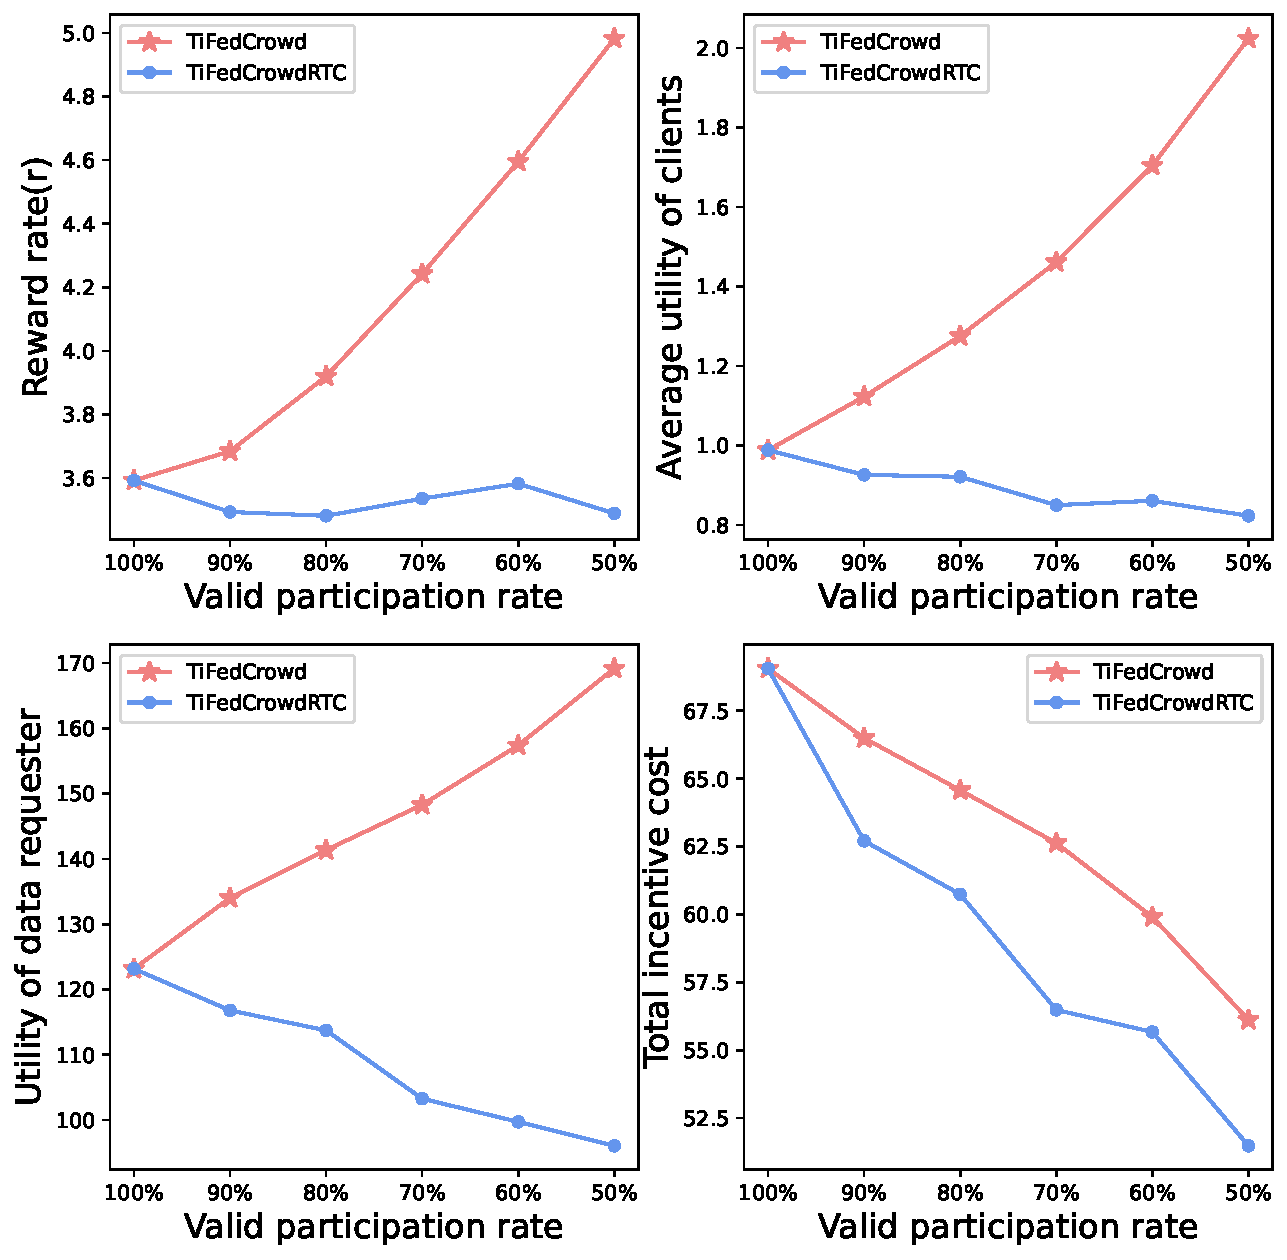
\includegraphics[width=5.5in]{fig3.pdf}}
	\caption{Reward rate ($r$), average utility of clients, utility of the server, and total incentive cost vs. valid participation rate.}
	\label{fig:3}
\end{figure}

Figure~\ref{fig:3} reveals the comparison between TiFedCrowd and RTC for the reward rate ($r$), the average utility of clients, the utility of the server, and the total incentive cost. Obviously, there is no difference in performance between TiFedCrowd and RTC when the valid participation rate reaches $100\%$. At this point, all uploaded models in TiFedCrowd are accepted by the server as in RTC. And other observations are as follows:

\lowercase{\romannumeral1}) There is little fluctuation of the reward rate ($r$) in the RTC with the change of different valid participation rates. However, in TiFedCrowd, the reward rate ($r$) increases as the valid participation rate decreases. According to Eq. (~\ref{eq:opt_r}), the reward rate ($r$) under the Nash equilibrium is only related to the number of valid participants $\zeta$ and the client parameter $\gamma$. Since the client parameters $\{\gamma_k\}_{k=1}^{30}$ are uniformly distributed on the interval $[0.5, 1.0]$, moreover, the number of valid participants $\zeta$ for RTC is always $30$, the reward rate ($r$) in RTC fluctuates only in a very small range. But the valid participants of TiFedCrowd become less and less as the decrease of valid participation rate, so incentives (e.g., the reward rate ($r$)) on the server-side need to be increased to encourage more clients to participate in federated crowdsourcing validly to collect enough data. 

\lowercase{\romannumeral2}) The lower the valid participation rate, the less the average utility of clients and the utility of the server in RTC but the more in TiFedCrowd. Because the lower the valid participation rate, the lower the average accuracy the clients contribute in RTC, which incurs a decrease both in the average reward received by the clients and the accuracy of the global model. Fortunately, TiFedCrowd has a time control mechanism to screen out and reject low-accuracy models by specifying the minimum completion time, so the average accuracy the clients contribute and the accuracy of the global model will not be reduced. For one thing, fewer valid participants lead to less total incentive cost on the server-side in TiFedCrowd thus increasing the utility of the server. For another thing, the decrease in the valid participation rate increases the reward rate ($r$) in TiFedCrowd, for which the average utility of clients increases. 

\lowercase{\romannumeral3}) The total incentive cost of both RTC and TiFedCrowd reduces with the decrease of effective participation rate. But the reasons for the decline are different. The reduction of the total incentive cost in TiFedCrowd is due to the decrease in the number of valid participants. While in RTC, the total incentive cost on the server-side reduces because the server accepts more low-quality data/models. 

\lowercase{\romannumeral4}) As long as the valid participation rate is less than $100\%$, the reward rate ($r$), the average utility of clients, and the utility of the server in TiFedCrowd are always higher than in RTC. The gap even grows as the valid participation rate decreases. In other words, as long as the valid participation rate does not reach $100\%$, TiFedCrowd always perform better than RTC. The time control mechanism in TiFedCrowd can effectively prevent malicious clients from submitting low-quality data/models in exchange for quick rewards, thus ensuring the quality of the final global model.

\subsection{Comparison Results on Multiple Heterogeneous Federated Crowdsourcing (MHFC) Tasks} \label{MHFC}

To verify that TiFedCrowd is also effective in the multiple heterogeneous federated crowdsourcing scenario, we compared the performance in MHFC between TiFedCrowd and baselines. We assumed that there were 3 heterogeneous federated crowdsourcing tasks $\{\Omega^{(1)},\Omega^{(2)},\Omega^{(3)}\}$. The number of clients participating in these three heterogeneous tasks was 15, 20, and 25, respectively. we set theInitialization parameters on the server-side for $\{\alpha^{(i)}\}_{i=1}^3 = \{200, 250, 300\}$ and $\beta=0$. Then the other parameters set the same as in the subsection~\ref{PCWB}.

\begin{figure}
	\centering
	\centerline{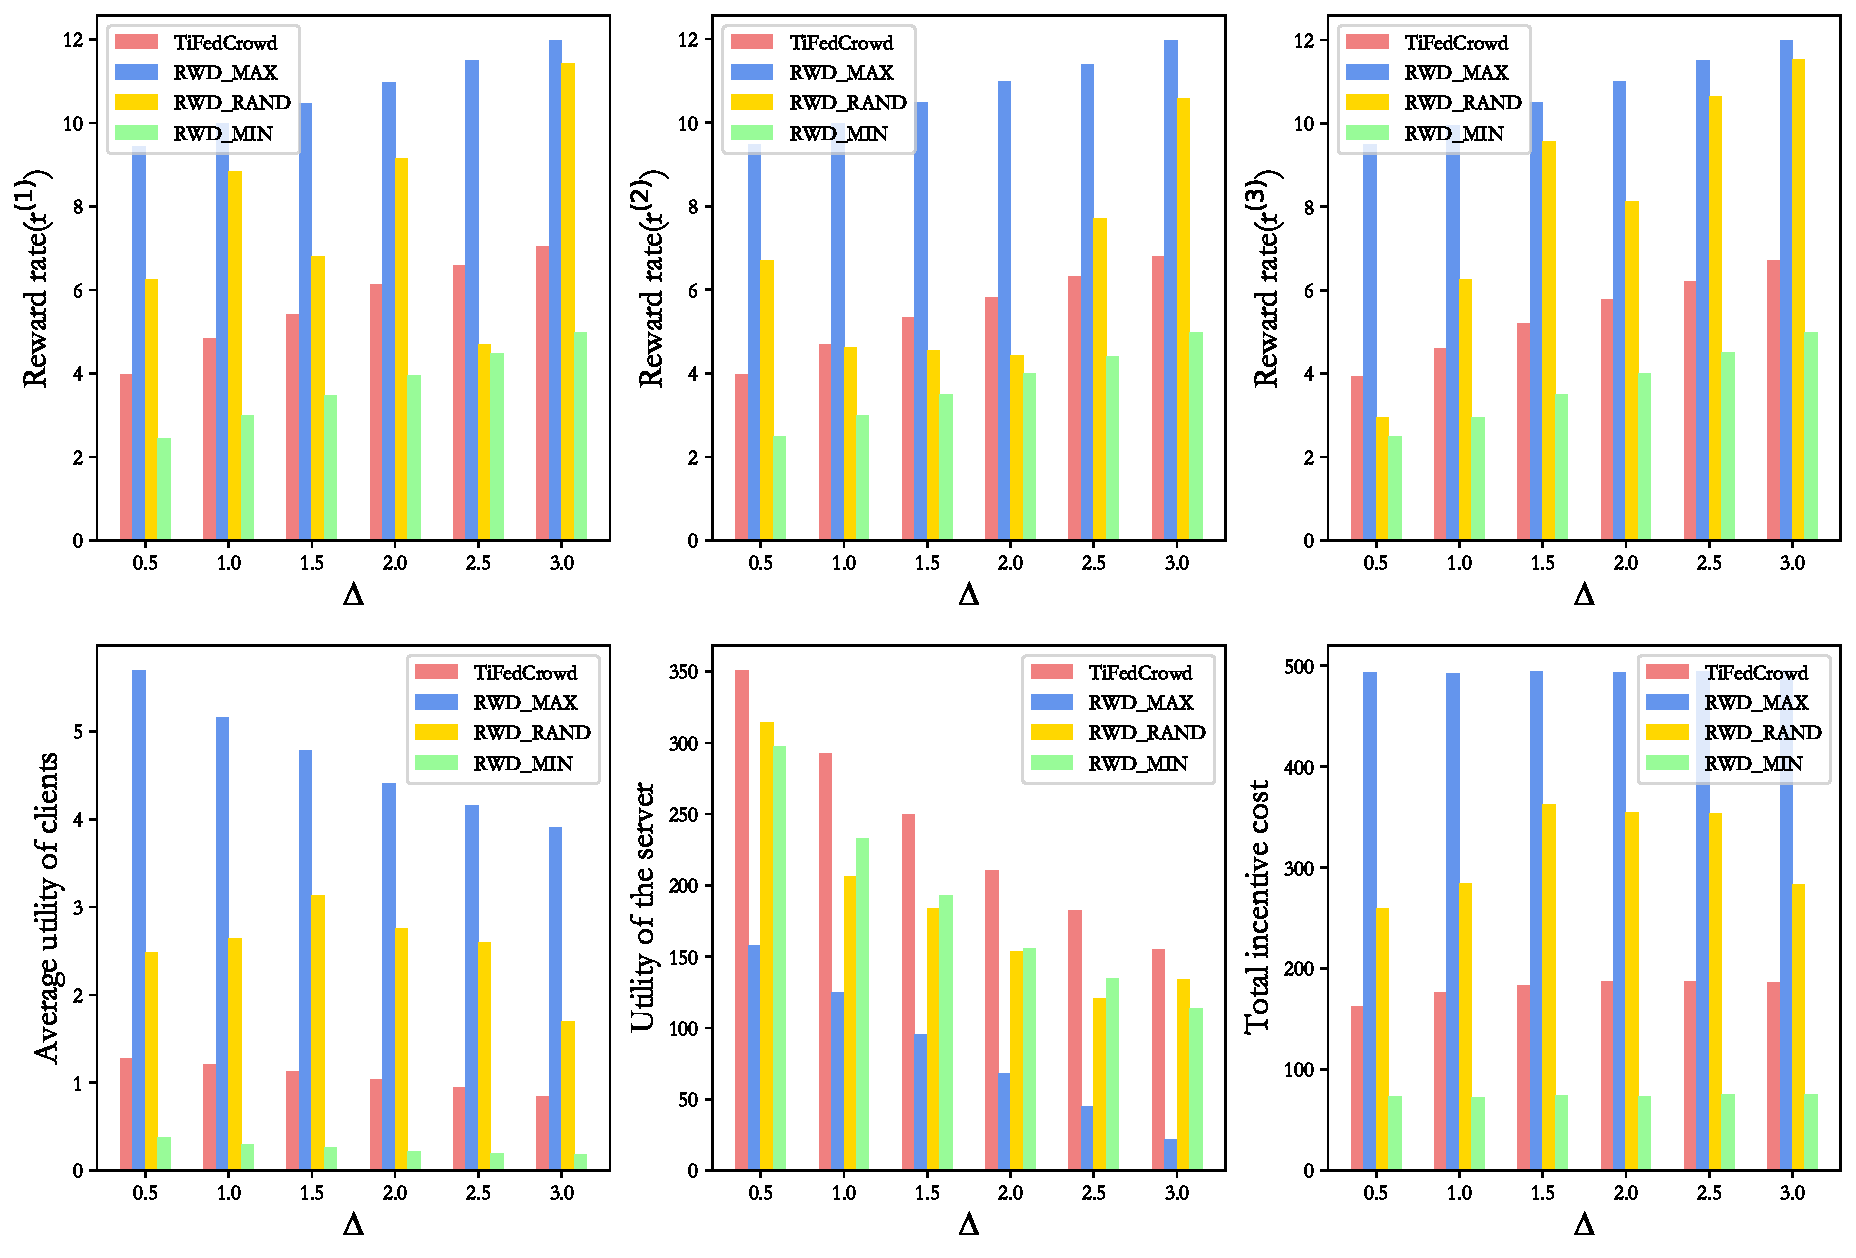
\includegraphics[width=5.5in]{fig5.pdf}}
	\caption{Reward rates ($\bm{r}$), average utility of clients, utility of the server, and total incentive cost vs. client parameter $\gamma$ ($\gamma\in[\Delta,\Delta+0.5]$) on MHFC.}
	\label{fig:5}
\end{figure}

Figure~\ref{fig:5} shows the comparison results for the reward rates ($\bm{r}$), the average utility of clients, the utility of the server, and the total incentive cost respectively between TiFedCrowd and the baselines on MHFC. We can observe results consistent with those in  subsection~\ref{PCWB}. 

\subsection{Experiment on a Real-World Dataset} \label{ERCP}
We used a short term heart rate prediction model of an LSTM-based model called FitRec \citep{ni2019modeling} for the experiment on a dataset named Endomondo \citep{ni2019modeling}, which containes data items including user identity, gender, sport, heart rate, timestamps, distance, speed, longitude, latitude, and altitude. Endomondo is a real-word dataset collecting data from the website endomondo.com. 

We set the number of clients to be $20$ and the valid participation rate to be $80\%$. Then, we let each client sample data at a random sequence of time intervals between 5 and 10 seconds. We measured the performance of the prediction tasks by the Root Mean Squared Error (RMSE).

\begin{table}
	%\renewcommand\arraystretch{1.5}
	\caption{Experimental results of prediction model FitRec on dataset Endomondo}
	\centering
	\resizebox{\textwidth}{16mm}{ 
	\begin{tabular}{cccccc} 
		\toprule
		& \textbf{ Reward rate ($r$) }  & \textbf{ Average utility of clients } & \textbf{ Utility of the server } & \textbf{ Total incentive cost } & \textbf{ RMSE }      \\ 
		\hline
		\textbf{ MAX }     & 9.487 & 5.687 & 128.315 & 131.617 & 3.059 \\
		\textbf{ MIN }    & 2.483 & 0.371 & 128.736 & 18.970 & 17.079 \\
		\textbf{ RANDOM }    & 5.987 & 3.115 & 152.032 & 81.325 & 4.577 \\
		\textbf{ TiFedCrow } & 4.905 & 1.907 & 163.568 & 57.961 & 3.422  \\
		\textbf{ RTC } & 4.376 & 1.420 & 135.191 & 55.686 & 5.611 \\ 
		\textbf{ iFedCrow }   & - & - & - &  & 5.912 \\
		\bottomrule
	\end{tabular}}
	\label{tab:t1}
\end{table}

The experimental results are shown in Table~\ref{tab:t1}. We have the following findings: \lowercase{\romannumeral1}) There is no doubt that RWD\_MAX makes the model perform best because it always motivates the clients to the maximum. Moreover, RWD\_MAX also makes the average utility of clients the highest. However, it minimizes the utility of the server, which is not cost-effective for the server-side. \lowercase{\romannumeral2}) Although the utility of the server in RWD\_MIN is higher than in RWD\_MAX, the model based on method RWD\_MIN has the worst performance. As we analyzed in subsection~\ref{ITNC}, RWD\_MIN maximizes the utility of the server by minimizing the total incentive cost on the server side. In addition, the comparison of model performance based on these two methods precisely demonstrates the necessity of theincentive mechanism for federated crowdsourcing. \lowercase{\romannumeral3}) The performance of the TiFedCrowd-based model is only slightly worse than the RWD\_MAX-based. However, TiFedCrowd makes the utility of the server far more than RWD\_MAX. It can be seen that RWD\_MAX causes a lot of waste of incentive cost on the server side. \lowercase{\romannumeral4}) Models based on RTC and iFedCrowd \citep{kang2022incentive} have similar performance. But they still perform slightly worse than RWD\_RAND-based model. Neither RTC nor iFedCrowd has a time control mechanism to filter out low-quality data. Obviously, the time control mechanism has a significant effect on improving the performance of the model. Besides, our TiFedCrowd is superior to iFedCrowd not only because of the time control mechanism in TiFedCrowd to screen out low-quality data but also because TiFedCrowd has a shorter computing time than iFedCrowd. The latter has been confirmed in subsection~\ref{CTCT}.

\section{Conclusion} \label{sec:con}
This paper proposes a novel incentive methodTiFedCrowd for the federated crowdsourcing scenario where workers participate in federated learning tasks under a privacy protection condition. TiFedCrowd models the federated crowdsourcing process where the server interacts with multiple clients as a two-stage Stackelberg game. At the same time, a time control mechanism is brought in TiFedCrowd, which restricts the time for clients to complete and submit federated crowdsourcing tasks. The time control mechanism not only initially filters out low-quality data/models but also allows the data requester to keep the data fresh and keep the maximum waiting time within an acceptable limit. This paper derives the Nash equilibrium of the two-stage Stackelberg game to obtain a global optimal solution, which makes the clients and the server in the competition maximize their utility concurrently. The TiFedCrowd method is easy to be extended to a multiple heterogeneous federated crowdsourcing scenario and still maintains its global optimal characteristics. A large number of experiments have demonstrated that TiFedCrowd can facilitate crowd workers to efficiently complete federated learning tasks with high quality using the smallest possible budget and within the deadline provided by the data/model requester. In the future, we will further explore how a client chooses to complete the tasks in combination to maximize its utility within the allowed time in the case of a large number of heterogeneous tasks.

\section*{Acknowledgments}
This work was sponsored by the National Natural Science Foundation of China (No.62076130 and No. 61902186) and the Start-up Research Fund of Southeast University (No. RF1028623059).


\bibliography{ref}
\end{document}
